\chapter{Parallel Computing}

The popularity of computational chemistry can be attributed in no small part to the advances and devlopment of highly efficient algorithms in theoretical chemistry. Equally important however is the ever increasing accessibility and performance of computing resources: commercially available work stations can handle chemical systems which could only be modelled on supercomputers a couple decades ago, and firmly cemented the position of computational chemsitry as an important "experimental" tool in the toolbox of a chemist. 

As the speed of computers increased over the years, so did the complexity of their components. Nowadays, programmers can choose between several types of architectures, such as shared or distributed memory systems, or accelerators like GPUs. Knowing the strenths and weaknesses of each type is paramount to developing efficient algorithms and tackling larger molecular systems.

This chapter gives an overview on computer architecture, and the different types of parallelism encountered on modern hardware.

\section{Moore's Law}

\emph{Moore's Law} states that the transistor density in integrated chips doubles every 12 to 24 months. First formulated in 1965 by Gordon More, his prediction has held up fairly well over the years. However, the technology enabling this trend has changed over the years.

Figure ... shows the trends in clock speed, single-thread performance, power consumption and number of logical cores and transistors for microprocessors from 1970 to 2000. Since the early 2000s, clock-speed and single-thread performance have begun to plateau, and have stagnated from 2010 onwards. Increasing the clock speed to values beyond 4 to 5 GHz generates too much stress on the microchip in form of heat, and decreases its performance. This flaw was compensated by using the growing transistor density to instead increase the number of logical cores on a single chip. 

Shifting towards increasing core count however entails that the most ideal perfpormance of a CPU can only be achieved though parallel programming. With the rise of parallel computing, the number of different parallel hardware features drastically increased, and it can be difficult for programmers to fully exploit the available computing resources. Moreover, different programming language and compiler extensions have emerged alongside, with numerous competing standards, especially for GPUs. 

\begin{figure}
\centering
\includegraphics[scale=1.2]{Pics/moore}
\caption{Taken from \protect\url{https://github.com/karlrupp/microprocessor-trend-data}}
\end{figure}

\subsection{Benefits and Limits of Parallel Computing}

While the different available programming models can seem daunting at first, one of the major advantages of parallel computing is improved \emph{scalabilty}. An application that exposes parallelism can be sped up by several orders of magnitude, simply by adding more compute power, with several different architectures to choose from. The limit of what problem sizes can be tackled is mostly dictated by the \emph{amount} of available computing resources and storage, rather than individual processor charcterstics.

As important as parallel computing has become in recent years, there is a reason why increasing clock speed was seen as the foremost strategy in keeping Moore's law alive. First, modifying a serial program to exploit parallelism can be a time-consuming endeavour, and second, not all tasks can be effectively parallelized. This means that the potential amount of seed-up is limited by the amount of parallel code. This is known as \emph{Amdahl's law}. The speed-up for a number of cores $N_c$ is given by
\begin{equation}
Speed-Up(N_c) = \frac{1}{S + \frac{P}{N_c}}
\end{equation}
\noindent where $S$ is the fraction of serial code and $P$ is the fraction of parallel code. The speedup for a fixed-size problem as a number of cores is known as \emph{strong scaling}, and the time-to-solution on each indivual core \emph{decreases} when more cores are added.

An alternate way to compute potential speed-up is given by Gustafson-Barsis's Law
\begin{equation}
Speed-Up(N_c) = N_c - S(N_c-1)
\end{equation}
\noindent where the problem size also increases proportionally to the number of cores. The scaling for this trend is known as \emph{weak scaling}. In this scenario, the time-to-solution spend on each core remains constant, as the system size and number of cores increases. Even if this type is called \emph{weak}, both forms of scaling are equally important, as they adress different scenarios.  

Why parallel computing?
-> becomes increasingly important, programmers should be well versed in it

Moores's Law

Fundamental law's: Amdahl

Types of parallelism:
- vectorization
- threads
- processes
- streaming (GPU)

Work at different levels of hardware

SETI@HOME

Categorizing parallel approaches Flynn's Taxonomy

errors in parallelism (p.40-41)

Performance limits
Levels of memory : speed vs feed (p. 59) show example of sizes of L caches

\begin{figure}
\centering
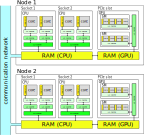
\includegraphics[scale=1.0]{Pics/memory}
\caption{Memory hierarchy}
\end{figure}